\chapter{Dunnville sandstone}\label{ch3:title}


This chapter presents a summary of geology, mineralogy and mechanical properties of Dunnville sandstone. The results of simple tests such as uniaxial compression test and conventional triaxial tests on dry specimens are discussed and analyzed.

\section{Geology, mineralogy and properties of the Dunnville sandstone}

In this study, Dunnville sandstone was selected for the laboratory experiments due to its availability, homogeneity and its isotropic behavior (at high mean stress when cracks are closed). Indeed, previous experiments on Dunnville Sandstone showed an isotropic behavior under different conditions of triaxial testing \cite{Tarokh2016}. The following paragraphs provide a short summary of geological and mineralogical properties of Dunnville sandstone.

\subsection{Geological history}

Dunnville sandstone comes from Dunnville, Wisconsin. The quarry is located in a valley at the intersection of the Chippewa river and one of its tributary. Dunnville sandstone constituent materials were deposited during the Cambrian period when Wisconsin was submerged several times by a sea, enabling the deposition of a large amount of sediments. The consolidation and compaction of the deposited materials by glaciers during the Pleistocene Epoch geological time and the subsequent removal of ice due to melting and rise in ambient temperatures led to the development of highly over-consolidated sedimentary rocks in the region (i.e., Dunnville sandstone). Dunnville sandstone is a member of the Elk Mount Formation and particularly the Eau Claire group \cite{Ostrom1966}.

\subsection{Mineralogy}

Dunnville Sandstone is composed of 90\% of medium-grained quartz and a small amount of cementitious material and may be referred to as a quartz arenite. Other minerals are readily noticeable such as orange beds of alkali feldspars and biotite grains (Fig. \ref{fig3:1}). The elongated biotite crystals are disparately distributed in the rock matrix and oriented parallel to the bedding. The mineralogical composition of Dunnville sandstone performed by American Engineering Testing is summarized in Table \ref{tb3:mineralogy} \cite{Tarokh2016}. Dunnville sandstone is a highly porous and permeable rock, with a porosity of 29-30\% and permeability of 220 mD \cite{Tarokh2016}.

\begin{figure}[tb]
    \centering
    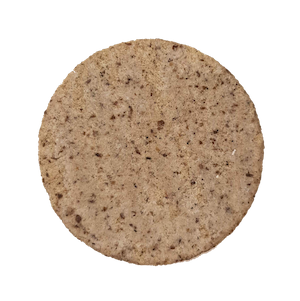
\includegraphics[width=0.4\columnwidth]{ch3/20191016_151842}
    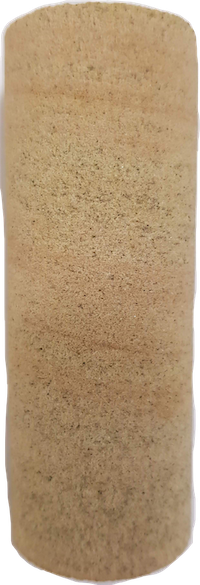
\includegraphics[width=0.15\columnwidth]{ch3/20191017_105210}
    \caption{Dunnville sandstone mineralogy}
    \label{fig3:1}
\end{figure} 

\begin{table}[h]
    \centering
    \captionsetup{justification=centering}
    \caption{Mineralogy of Dunnville Sandstone \cite{Tarokh2016}}
    \begin{tabular}{lc} \hline
        Mineral & Volume [\%] \\ \hline \hline
        Quartz & 90-95 \\ 
        Alkali Feldspar & 2-5 \\ 
        Biotite & 2-5 \\ 
        Plagioclase & Trace -1 \\ 
        Muscovite & Trace \\ 
        Clinozoisite & Trace \\ 
        Zircon & Trace \\ 
        Hematite & Trace \\ 
        Iron-oxide & 1-2 \\ \hline
    \end{tabular}
    \label{tb3:mineralogy}
\end{table}

The dry density and the P-wave velocity  were measured for all specimens tested in this study. The dry density $\rho$ is $1910 \pm 30 \; \text{kg/m}^3$ and the P-wave velocity $V_P$ is $1825\pm 124 \; \text{m/s}$ . The wave travel time for evaluation of the P-wave velocity was measured perpendicular to the bedding planes.

\section{Uniaxial compression test}

One uniaxial compression test was performed on Dunnville sandstone to determine Young’s modulus $E_i$ and the uniaxial compressive strength $C_o$. These parameters are essential to understand the behavior of the rock and are used for the analysis of behavior in subsequent chapters.

\subsection{Specimen preparation}

A cylindrical specimen was ground to ensure the ends were perpendicular to the specimen axis and dried prior to test in accordance with the ISRM suggested methods \cite{ISRM2015} and ASTM standard \cite{ASTM2019}. A detailed description of the specimen preparation procedure will be presented in section \ref{ch3:specimen-prep}. The specimen dimensions, with $h\approx 2d$, were: $h = \SI{95.70}{\milli\meter}$, $d = \SI{50.76}{\milli\meter}$. Following Labuz and Bridell (1993) \cite{Labuz1993}, stearic acid was applied to the specimen ends to reduce friction and thereby to minimize the end effects.

\subsection{Procedure}

The test was performed using a \SI{1}{\mega\newton} MTS closed loop servo-hydraulic load frame (MTS System Corporation). The uniaxial compression test was stroke controlled to avoid sudden failure of the rock where a displacement rate of \SI{0.001}{\milli\meter\per\second} was used. The displacement of the actuator (stroke) and the force applied to the specimen were recorded during the test.

A small seating load of $\sim 1-\SI{2}{\kilo\newton}$ was applied before the test initiated to ensure adequate contact between the loading platens and the specimen. The axial load was then increased until $\sim 50\%$ of the expected uniaxial compressive strength $C_0$ of the rock following by unloading to $\sim 1-\SI{2}{\kilo\newton}$. This loading-unloading cycle is used to determine the Young’s modulus $E_i$ of the rock after specimen displacements were corrected for the machine displacement. The axial load was then increased until failure of the rock specimen was achieved. The test was continued until the load decreased to $\sim 75\%$ of $C_0$. 

The following stress path describes the uniaxial test: 

\begin{equation}
    \sigma_1 = \sigma_a \text{ with } \sigma_a > 0
\end{equation}
\begin{equation}
    \sigma_2 = \sigma_3 = \sigma_r   \text{ with } \sigma_r = 0
\end{equation}
    

\subsection{Results}

From the recorded axial displacement and force, the axial stress and the axial strain can be computed: 

\begin{align}
    \sigma_a &= \frac{F_a}{A} \\
    \epsilon_a &= \frac{u}{h}
\end{align}

Where:

\begin{description}
    \item[$\sigma_a$] : axial stress  [\si{\mega\pascal}]
    \item[$\epsilon_a$] : axial strain [-]
    \item[$A=\frac{d\pi^2}{4}$] : cross section area of the cylindrical specimen [\si{\milli\meter\squared}]
    \item[$F_a$] :  axial load applied through the load frame [\si{\newton}]
    \item[$u$] : axial displacement corrected for machine displacement [\si{\milli\meter}]
    \item[$h$]  length of the specimen [\si{\milli\meter}]
\end{description}

Fig \ref{fig3:2} present the stress-strain plot obtained from the uniaxial compression test. The uniaxial compressive strength of the rock specimen is calculated as: 


\begin{figure}[p]
    \centering
    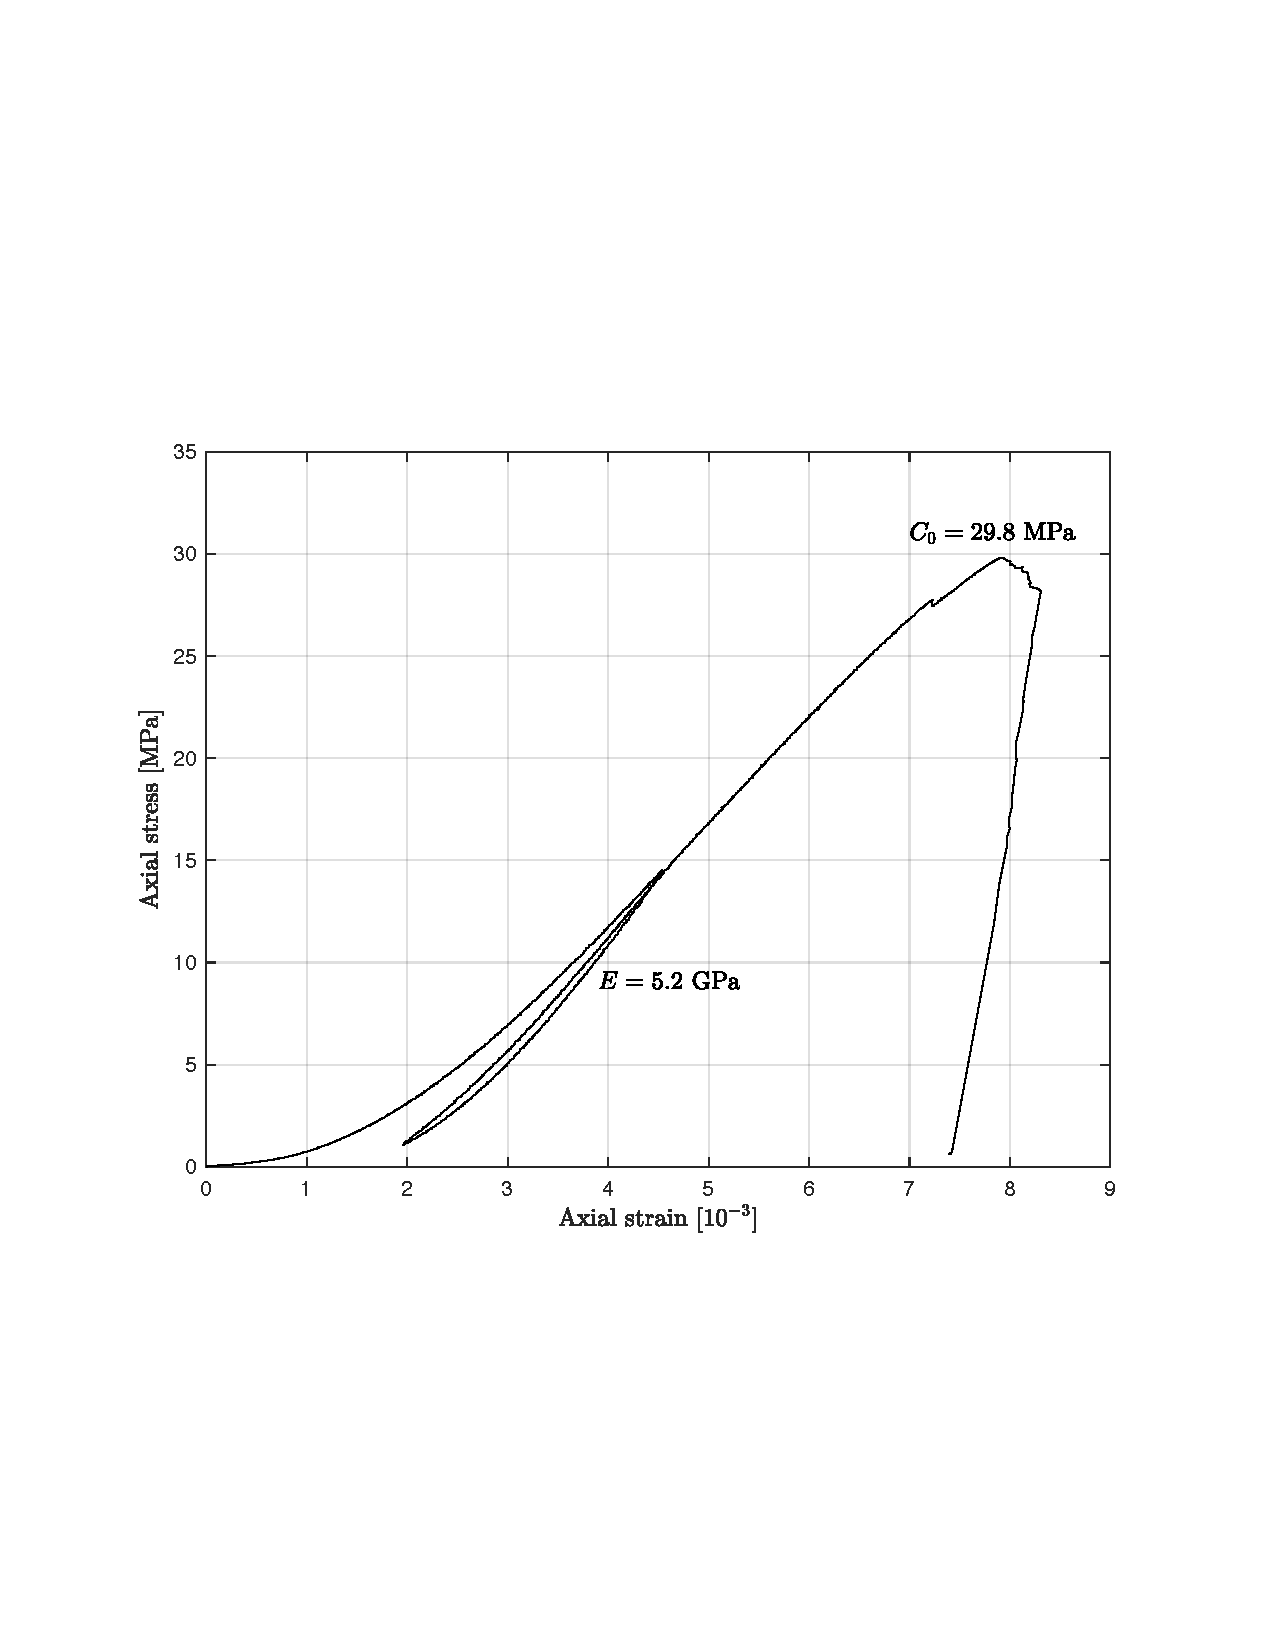
\includegraphics[width=0.9\columnwidth]{ch3/ucs.pdf}
    \caption{Stress and Strain relationship for the uniaxial compression test}
    \label{fig3:2}
\end{figure} 

\begin{equation}
    C_o = \frac{F_\text{peak}}{A} = \sigma_{a,\text{peak}} = \SI{29.83}{\mega\pascal}
\end{equation}

Young’s modulus of the rock is computed using the loading-unloading cycle:

\begin{equation}
    E=\frac{\Delta\sigma}{\Delta\epsilon} = \SI{5860}{\mega\pascal}
\end{equation}

Fig \ref{fig3:3} presents the specimen after the test. The failed specimen showed axial splitting and a failure surface with a conical shape. 

\begin{figure}[p]
    \centering
    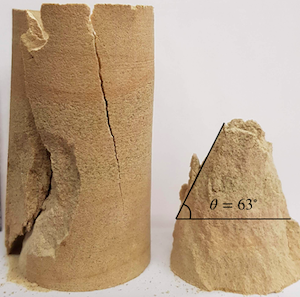
\includegraphics[width=0.4\columnwidth]{ch3/ucs.png}
    \caption{Failed specimen after the uniaxial compression test}
    \label{fig3:3}
\end{figure} 

\section{Conventional triaxial tests}\label{Conventional_Triaxial_tests}

Shear strength of Dunnville sandstone was determined using conventional (axisymmetric) triaxial tests (CT). Two types of CT tests were performed, namely, the conventional triaxial compression (CTC) and the conventional triaxial extension (CTE). For these tests, two of the principal stresses are equal. The state of stress of the rock specimen is then simplified to the axial stress $\sigma_a$ and the radial stress $\sigma_r$. 

\subsection{Hoek-Franklin cell}

A Hoek -Franklin pressure cell was used to perform the conventional triaxial tests \cite{Franklin1970}. The maximum capacity of the cell is \SI{69}{MPa} and allows the independent application of axial and radial stresses. The device is composed of a pressure vessel, a synthetic rubber membrane and two loading platens (Fig \ref{fig3:4}).

\begin{figure}[tb]
    \centering
    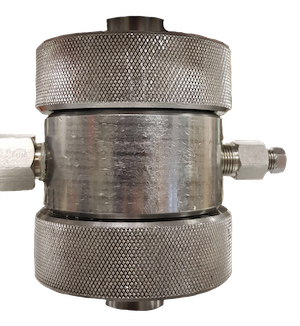
\includegraphics[width=0.4\columnwidth]{ch3/hoekcell}
    \caption{Hoek-Franklin cell}
    \label{fig3:4}
\end{figure} 

The radial stress was applied using a fluid pressure system where confinement is provided using hydraulic oil. The fluid pressure system is composed of a microcontroller and a screw-type hydraulic intensifier that allows for confining pressure to be held constant throughout the test. The axial load is applied through steel platens with a \SI{1}{\mega\newton} MTS servo-hydraulic load frame (MTS System Corporation). The monitoring of the axial displacement and axial force are done using a data acquisition system (Fig \ref{fig3:5}).

\begin{figure}[tb]
    \centering
    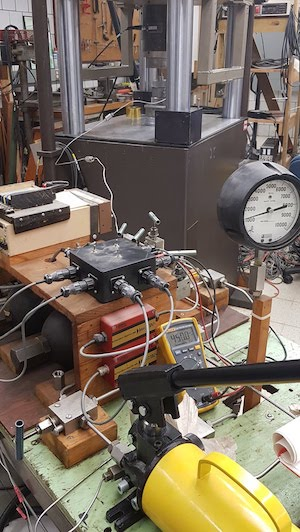
\includegraphics[width=0.4\columnwidth]{ch3/20190927_172117}
    \caption{Conventional triaxial test set up}
    \label{fig3:5}
\end{figure} 

A rubber membrane was used to isolate the specimen and the loading platens from the confining fluid, and to allow for radial and axial stresses to be applied independently. The membranes used herein have an inner diameter of \SI{32.0}{mm} and are \SI{85.0}{mm} in height (Fig \ref{fig3:6}).

\begin{figure}[tb]
    \centering
    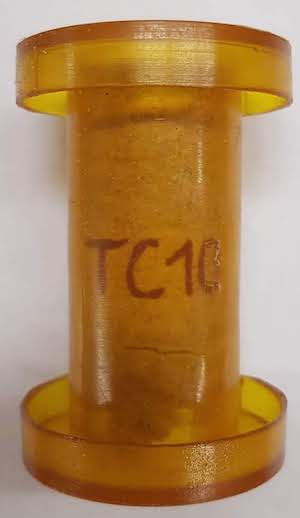
\includegraphics[width=0.3\columnwidth]{ch3/ctc10}
    \caption{Membrane hosting the rock specimen in the Hoek-Franklin cell}
    \label{fig3:6}
\end{figure} 

\subsection{Specimen preparation} \label{ch3:specimen-prep}

Rock cores were obtained from a block of Dunnville sandstone. The specimens were prepared following ASTM Standard Practice D4543-19 \cite{ASTM2019}. In preparation of the test specimens, particular attention was given to (i) the straightness of the elements on the cylindrical surface, (ii) flatness of the end bearing surfaces and (iii) perpendicularity of the end surfaces with the respect to axis of the core. The following describes the procedure used in preparation of the specimens:

\begin{enumerate}
    \item \emph{Cutting and grinding of the end surfaces}: for the purpose of sealing, the specimen dimensions should match that of the cell membrane. The core diameters ranged from \SIrange{30.2}{30.6}{mm}. The specimens were cut using a diamond saw and ground using a carborundum grinding wheel. A precision table was used to ensure that specimen ends were perpendicular to the specimen axis. The final height h of the specimens ranged from \SIrange{75.7}{81.8}{mm} 
    \item \emph{Drying}: all the specimens were oven dried at \SI{150}{\celsius} for at least 24 hours before the tests to ensure dry conditions existed during the triaxial tests
    \item \emph{Minimizing end friction}: the ends and cylindrical surface of the specimens were coated with stearic acid \cite{ASTM2019}. This lubricant was used to reduce frictional effects between the membrane and the specimen.
\end{enumerate}

In addition to standard preparation, one specimen (TC 9 at $\sigma_r = \SI{5.0}{MPa}$) was equipped with a strain gages rosette where axial and transverse strains were measured (Fig \ref{fig3:7}). The procedure for gluing the strain gage set was executed with much care to avoid damaging the gages. All the tools used in the process were cleaned with acid and neutralizer before touching the strain gage. Due to the high porosity of the Dunnville sandstone, the surface of the rock was coated with the same epoxy that was used to attach the gage. The surface of the specimen was then cleaned using xylene and the strain gage was attached using M-Bond 200 epoxy adhesive.

\begin{figure}[tb]
    \centering
    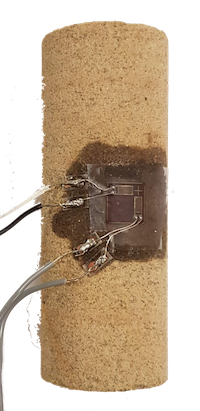
\includegraphics[width=0.25\columnwidth]{ch3/straingage.png}
    \caption{Strain Gage set up on a CTC specimen}
    \label{fig3:7}
\end{figure} 

\subsection{Conventional triaxial compression test} \label{ch3:Conventional-Triaxial-Compression-test}

The following procedure was followed to setup and conduct the conventional triaxial compression tests:

\begin{enumerate}
    \item The specimen was inserted in the Hoek-Franklin cell. The cell was held in a horizontal position and hydraulic oil was inserted to ensure no entrapped air existed in the annulus between the cell walls and the membrane.
    \item The pressure cell-specimen-loading platen assembly was then placed inside the load frame and seating stress of  $\sigma_a \approx \SI{1}{MPa}$ was applied to the specimen to ensure adequate contact between the specimen and the platens. To ensure small deviatoric stresses, $\sigma_r \approx \SI{1}{MPa}$ was applied. It is noted that this condition corresponds to a hydrostatic stress state ($\sigma_a = \sigma_r = \SI{1}{MPa}$ ).
    \item The axial ($\sigma_a$) and radial ($\sigma_r$) stresses were then increased hydrostatically until the desired confining pressure ($\sigma_r$) was achieved. In so doing, a stress increment of $\sim \SI{5.0}{MPa}$ was consistently used.
    \item Once the desired radial pressure $\sigma_r$ was reached, the deviatoric loading was initiated by maintaining the radial stress ($\sigma_r$) constant while axial stress ($\sigma_a$) were increased until failure was achieved. It is noted that all tests were stroke controlled with a displacement rate of \SI{0.001}{\meter\per\second}. The stress path applied during the test can be summarized as follow:
\end{enumerate}
\begin{equation}
    \sigma_1 = \sigma_a \text{ with } \sigma_a > 0
\end{equation}
\begin{equation}
    \sigma_2 = \sigma_3 = \sigma_r   \text{ with } \sigma_r = 0 
\end{equation}
\begin{equation}
    \sigma_a > \sigma_r
\end{equation}

\subsection{Conventional triaxial extension test}

The following procedure was followed to setup and run the conventional triaxial extension tests:

\begin{enumerate}
    \item The same device and tests preparation, as those previously explained for the conventional triaxial compression tests, were used for the conventional triaxial extension tests (see steps 1-3 in Section \ref{ch3:Conventional-Triaxial-Compression-test}).
    \item In a conventional triaxial extension test, however, the axial stress is decreased as opposed to increasing the axial stress in triaxial compression tests. 
    \item This test was stroke controlled with displacement rate of \SI{0.001}{\meter\per\second}. The radial stress was kept constant at the desired confining pressure using the hydraulic intensifier, while the axial stresses decreased through the displacement of the load frame. The stress path applied during the test can be summarized as follow:
\end{enumerate}
\begin{equation}
    \sigma_1 = \sigma_2 = \sigma_r  \text{ with } \sigma_r = 0 
\end{equation}
\begin{equation}
    \sigma_3 = \sigma_a \text{ with } \sigma_a < 0  
\end{equation}
\begin{equation}
    \sigma_a < \sigma_r
\end{equation}

\subsection{Results}

Five conventional triaxial compression tests ($\sigma_r =  5,10,20,40$ and $\SIlist{60}{MPa}$) and three conventional triaxial extension tests ($\sigma_r = 35,40$ and $\SIlist{60}{MPa}$) were performed. The test results are summarized in Table \ref{tb3:CTC-CTE-results} and the stress-strain relationships for all tests are shown in Fig \ref{fig3:8}

\begin{table}
    \centering
    \captionsetup{justification=centering}
    \caption{Summary of CTC and CTE tests results}
    \begin{tabular}{cccccccc}
        \hline 
        Test & $\sigma_1$ [\si{MPA}] & $\sigma_2$ [\si{MPA}] &$\sigma_3$ [\si{MPA}] & $p$ [\si{MPA}] & $q$ [\si{MPA}] & $\theta$ [\si{\degree}] & $E_i$ [\si{MPA}] \\
        \hline
        \hline
        TC 9  & 49.43 & 5  & 5    & 19.81 & 44.43 & 0  & 5861  \\ 
        TC 0  & 61.43 & 10 & 10   & 27.95 & 51.43 & 0  & 6407  \\ 
        TC 5  & 91.08 & 20 & 20   & 44.72 & 71.08 & 0  & 7014  \\ 
        TC 8  & 127.3 & 40 & 40   & 65.73 & 87.30 & 0  & 6687  \\ 
        TC 10 & 151.1 & 60 & 60   & 88.12 & 91.10 & 0  & 6842  \\ 
        \hline
        \hline
        TE 3  & 35    & 35 & 3.96 & 24.64 & 31.08 & 60 & 7922  \\ 
        TE 1  & 40    & 40 & 4.50 & 27.89 & 36.34 & 60 & 8390  \\ 
        TE 2  & 60    & 60 & 9.68 & 43.01 & 50.98 & 60 & 8695  \\
        \hline
    \end{tabular}
    \label{tb3:CTC-CTE-results}
\end{table}

\begin{figure}[p]
    \centering
    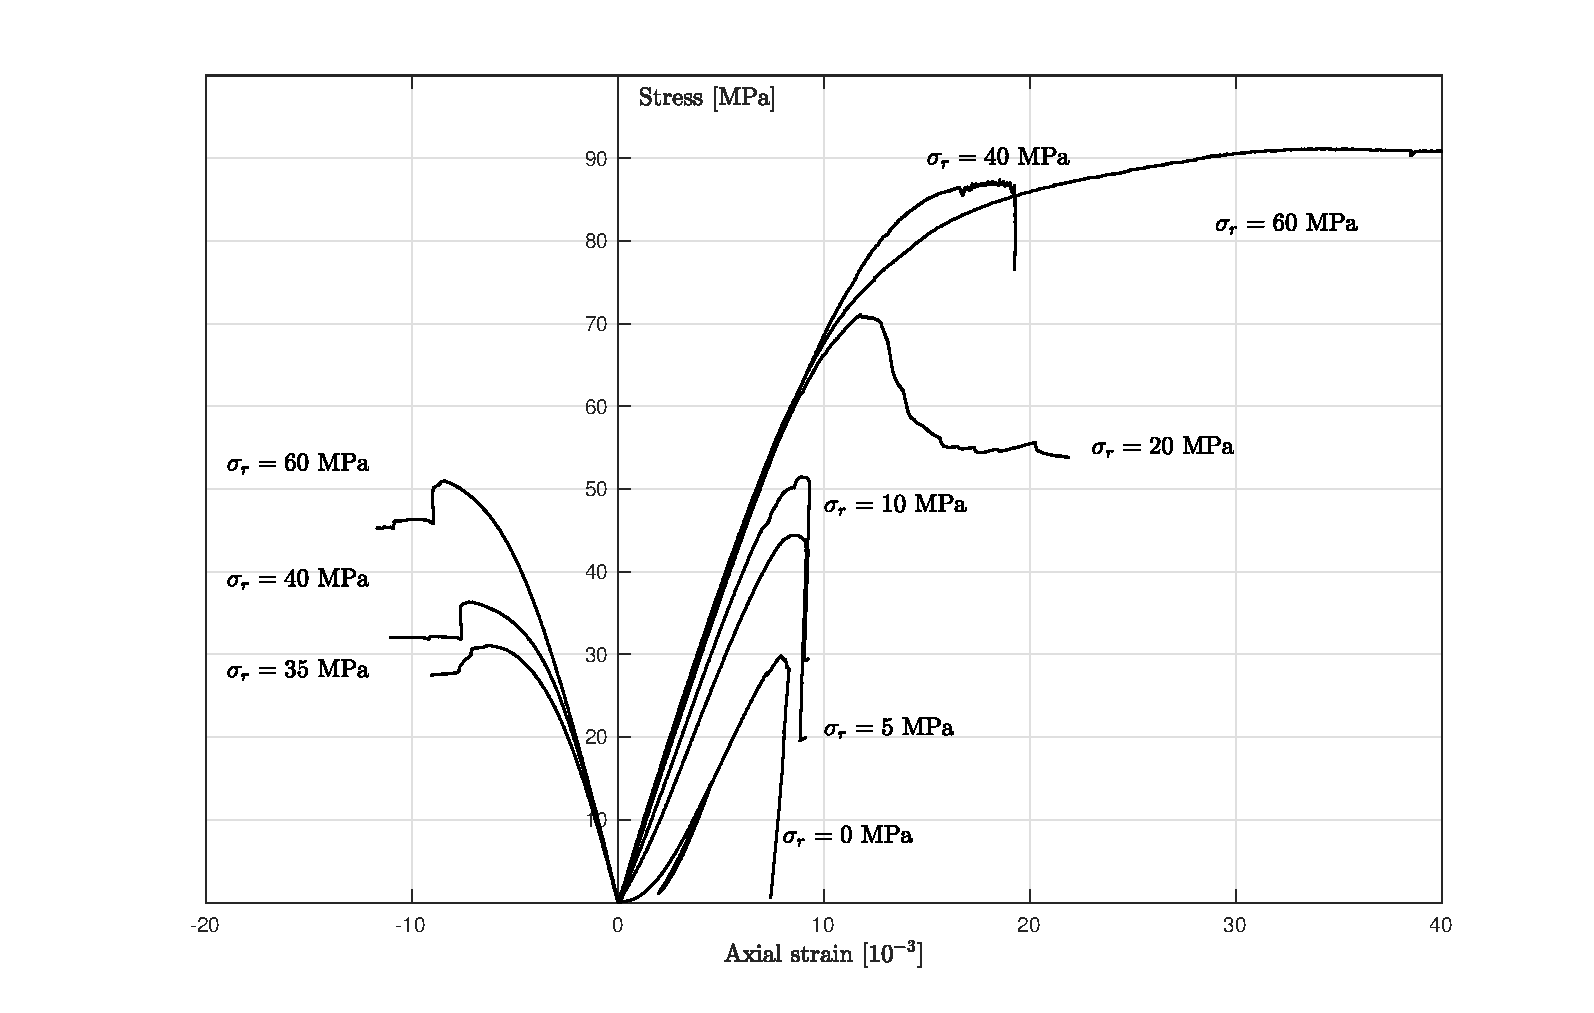
\includegraphics[width=\columnwidth]{ch3/StressStrain_summ1}
    \caption{Summary of the stress-strain relationships for the triaxial compression and extension tests}
    \label{fig3:8}
\end{figure} 

\subsubsection{Conventional triaxial compression tests}

\paragraph{Stress vs. strain plot}
From \SIrange{0}{20}{MPa} of confining stress, the rock is in the brittle domain as the axial stress is dropping after reaching maximal axial stress. At higher confining pressures ($\sigma_r > \SI{40}{\mega\pascal}$ and $\sigma_r < \SI{60}{\mega\pascal}$), however, rock is transitioning from a brittle to ductile response as represented by the post-peak drop in stresses as seen in Fig. \ref{fig3:8}. Finally, the rock shows a ductile behavior under a confining stress of \SI{60}{MPa}, were the axial stress does not reach a peak value.

\paragraph{Mohr circles plot}
The conventional triaxial compression results can also be presented on a Mohr plane, where the Mohr circles and the non-linear failure envelope are shown (Figure \ref{fig3:9}). This plot indicates that the friction angle for Dunnville sandstone is stress dependent and cannot be represented using the Mohr-Coulomb linear failure envelope for the entire range of possible stress states. The nonlinear failure envelope, however, may be linearized over small stress intervals as shown in Fig \ref{fig3:9}. The corresponding Mohr-Coulomb strength parameters (friction angle $\phi$ and cohesion intercept $c$) are summarized in Table \ref{tb3:MC-param}.

\begin{table}[h]
    \centering
    \captionsetup{justification=centering}
    \caption{Mohr-Coulomb strength parameters for various stress regimes for Dunnville sandstone}
    \begin{tabular}{ccc}
        \hline
        Segment & [$\phi$ \si{\degree}] & $c$[\si{MPa}] \\
        \hline
        \hline
        5 – 10 MPa  & 30.73 & 9.67   \\ 
        10 – 20 MPa & 29.37 & 10.42  \\ 
        20 – 40 MPa & 14.41 & 23.6   \\ 
        40 – 60 MPa & 4.72  & 36.94  \\
        \hline
    \end{tabular}
    \label{tb3:MC-param}
\end{table}

\begin{figure}[hp]
    \centering
    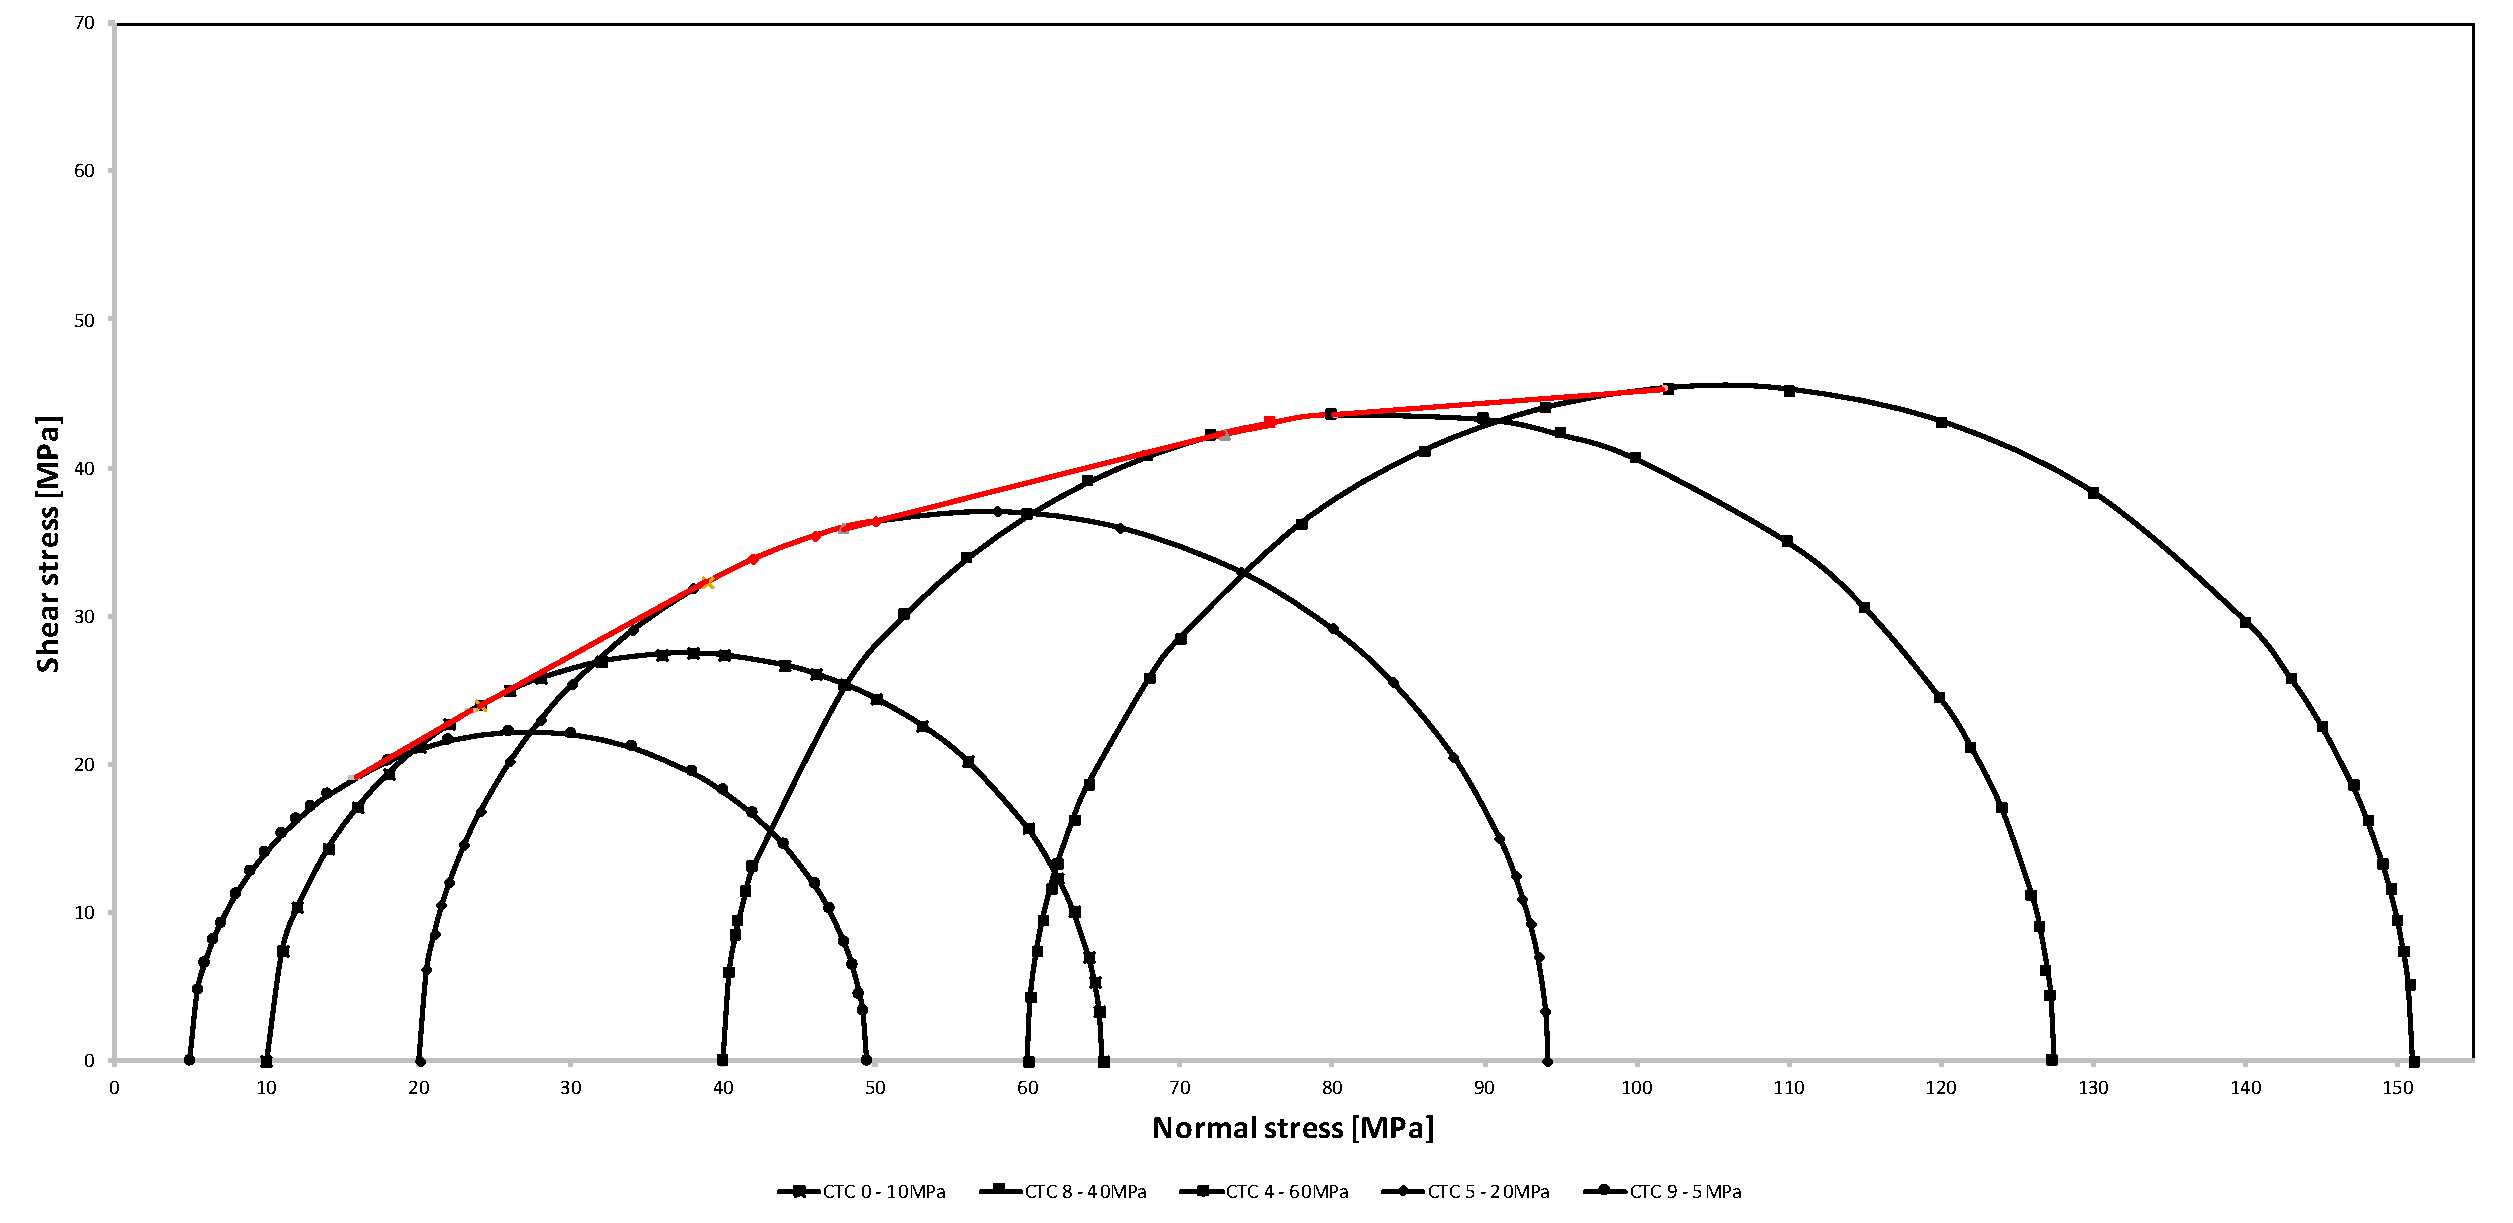
\includegraphics[width=\columnwidth]{ch3/mohrcoulomb}
    \caption{Mohr-Coulomb circles for the conventional triaxial compression tests.}
    \label{fig3:9}
\end{figure} 

\paragraph{Poisson’s ratio} 

Poisson’s ratio of Dunnville sandstone was computed using the results of the axial and radial strains for specimen TC 9:

\begin{equation}
    \nu = \frac{-\epsilon_{\text{radial}}}{\epsilon_{\text{axial}}} = 0.26
\end{equation}

Fig \ref{fig3:10} shows a plot of the radial strain vs. the axial strain measured during the test.

\begin{figure}[h]
    \centering
    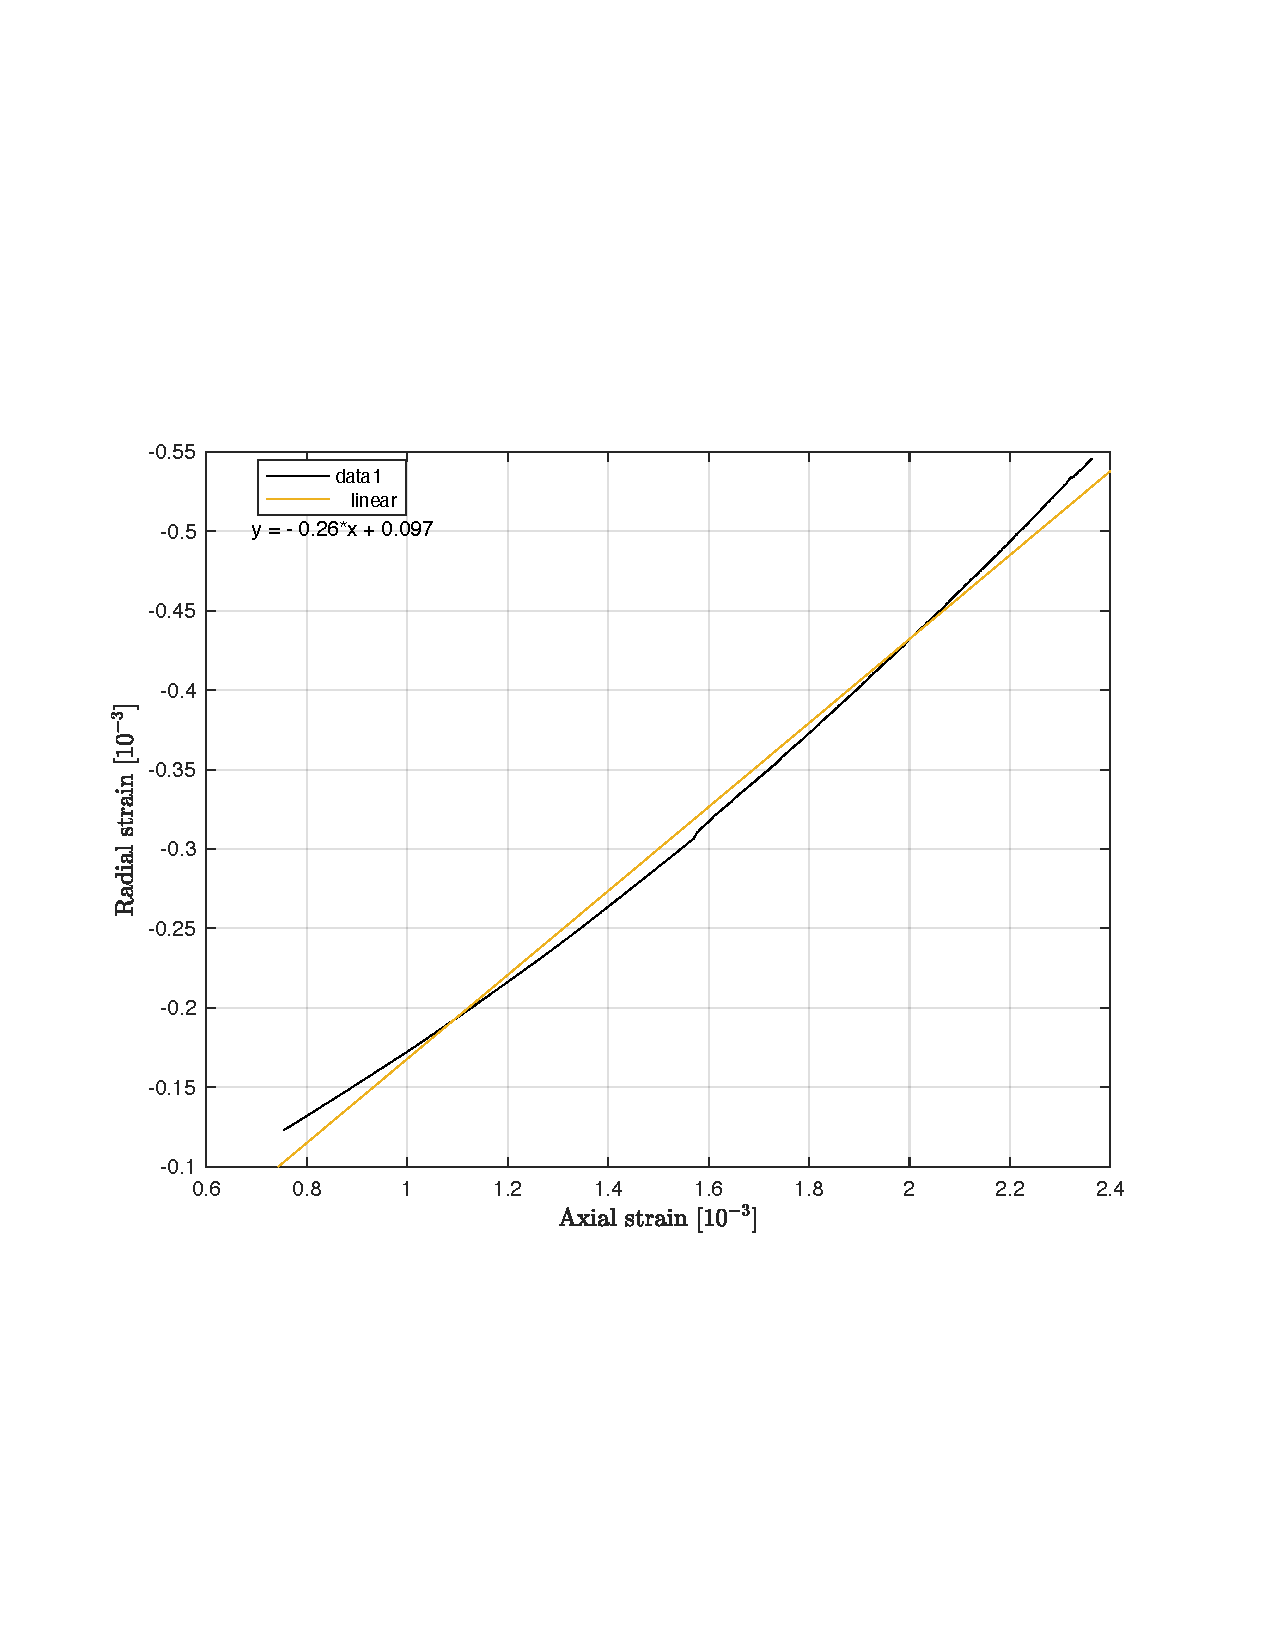
\includegraphics[width=0.9\columnwidth]{ch3/poisson}
    \caption{Poisson's ratio of Dunnville sandstone}
    \label{fig3:10}
\end{figure} 

\paragraph{Failure surfaces}

Table \ref{tb3:photoCTC} presents photos of the CTC tests specimens after failure, where the failure surfaces are observable. A majority of the specimens shows failure angles of approximately \ang{60}, corresponding to the Mohr-circles prediction of $45+\phi/2$. The specimen tested at a confining pressure of $\SI{60}{\mega\pascal}$ showed multiple horizontal bands. At this value of mean stress, the rock behavior becomes ductile, leading to the formation of compaction bands. 

\begin{table}
    \centering
    \captionsetup{justification=centering}
    \caption{Failure surfaces for conventional triaxial compression tests}
    \begin{tabular}{|c|c|c|c|c|}
     \hline
     $\sigma_r = \SI{5}{MPa}$ & $\sigma_r = \SI{10}{MPa}$ &  $\sigma_r = \SI{20}{MPa}$ & $\sigma_r = \SI{40}{MPa}$ & $\sigma_r = \SI{60}{MPa}$ \\
     \hline
     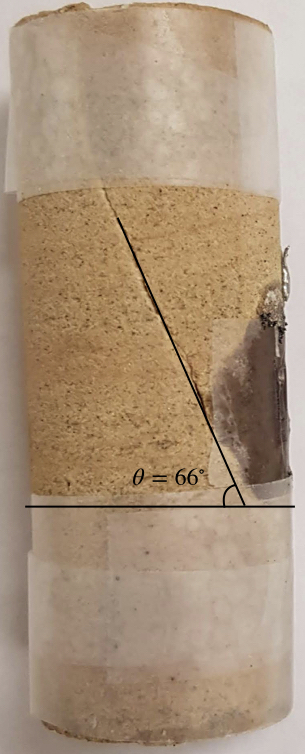
\includegraphics[width=0.15\columnwidth]{ch3/ctc9-001.jpeg} & 
     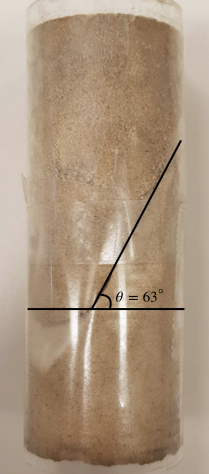
\includegraphics[width=0.17\columnwidth]{ch3/CT_failAng-001} &
     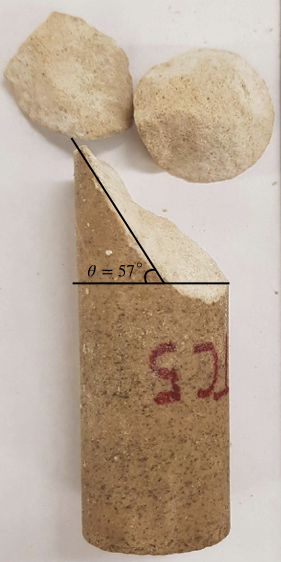
\includegraphics[width=0.19\columnwidth]{ch3/CT_failAng-002} &
     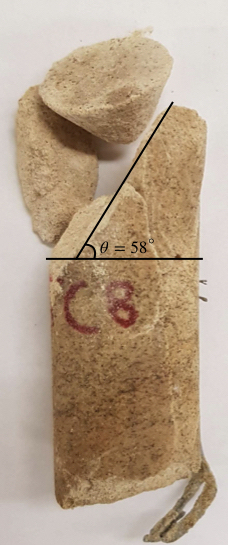
\includegraphics[width=0.16\columnwidth]{ch3/CT_failAng-003} &
     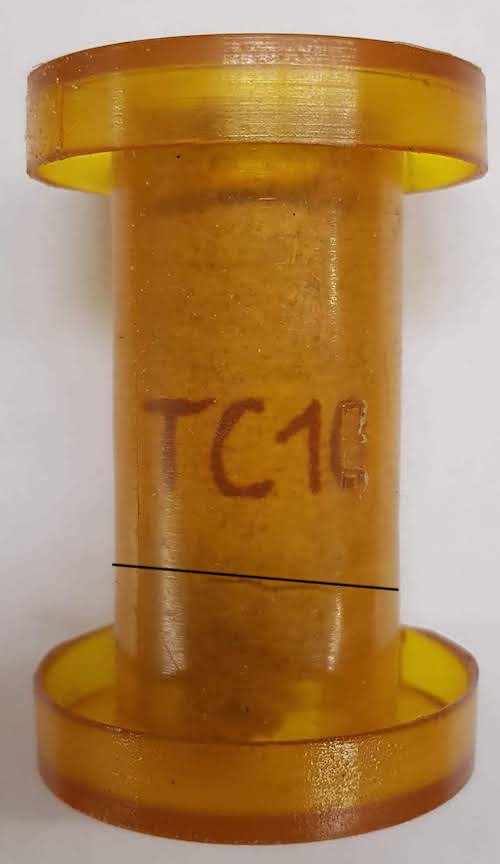
\includegraphics[width=0.2\columnwidth]{ch3/ctc10_tab} \\
     \hline
     $\theta = \ang{66}$ & $\theta = \ang{63}$  &  $\theta = \ang{57}$ & $\theta = \ang{58}$ & $\theta \simeq \ang{0}$ \\
     \hline
    \end{tabular}
    \label{tb3:photoCTC}
\end{table}

\subsubsection{Conventional triaxial extension tests}

\paragraph{Stress vs. strain plot}

Fig \ref{fig3:8} presents the axial stress vs. axial strain curves for the extension tests. The axial stress in the figure represent the amount of axial stress that is removed from the original hydrostatics state of stress. In order to find the axial stress at failure, the following formula is used: 

\begin{equation}
    \sigma_\text{failure} = \sigma_{a,\text{removed}} - \sigma_r
\end{equation}

\paragraph{Failure surfaces}

Table \ref{tb3:photoCTE} presents photos of the CTE tests specimens after failure. 


\begin{table}
    \centering
    \captionsetup{justification=centering}
    \caption{Failure surfaces for conventional triaxial extension tests}
    \begin{tabular}{|c|c|c|}
     \hline
     $\sigma_r = \SI{35}{MPa}$ & $\sigma_r = \SI{40}{MPa}$ &  $\sigma_r = \SI{60}{MPa}$ \\
     \hline
     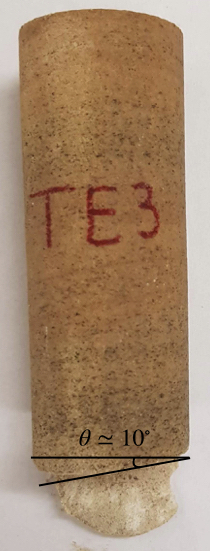
\includegraphics[width=0.2\columnwidth]{ch3/CTE_failAng-003} & 
     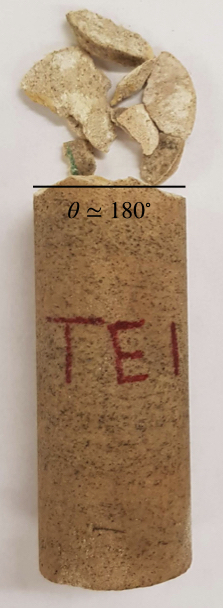
\includegraphics[width=0.2\columnwidth]{ch3/CTE_failAng-001} &
     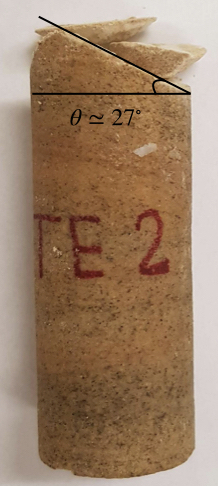
\includegraphics[width=0.2\columnwidth]{ch3/CTE_failAng-002} \\
     \hline
     $\theta = \ang{10}$ & $\theta = \ang{0}$  &  $\theta = \ang{27}$ \\
     \hline
    \end{tabular}
    \label{tb3:photoCTE}
\end{table}

